\documentclass{article}
\usepackage{graphicx}
\usepackage{amsmath}
%\usepackage{amssymb}
\usepackage{mathtools}
\usepackage{xcolor}
\usepackage{bm}

\usepackage{natbib}
\usepackage[hidelinks]{hyperref}
\usepackage{doi}
\usepackage{charter}
\usepackage[bitstream-charter]{mathdesign}
\usepackage[final,babel]{microtype}
\usepackage[utf8]{inputenc}
\usepackage[british]{babel}
\usepackage{csquotes}
\usepackage[T1]{fontenc}
\usepackage{makecell}
\usepackage{tikz}
\usetikzlibrary{arrows}
\usetikzlibrary{patterns}

\title{Thinking about 2D flow over a hill using Bernoulli's principle}
\author{James Shaw}
\date{25th April 2016}

\newcommand{\TODO}[1]{\textcolor{purple}{TODO: \emph{#1}}}

\begin{document}

\maketitle

Earlier in my PhD I studied gravity waves that were induced by flow over a hill in the two-dimensional test case by \citet{schaer2002} using a numerical model of the Euler equations \citep{shaw-weller2016}.  Bernoulli's principle states that, for incompressible steady-state flow in a pipe, energy is conserved along a streamline \citep{vallis2006}
\begin{align}
	\frac{\mathrm{D}}{\mathrm{D}t} \left( \underbrace{\frac{1}{2}\bm{u}^2}_\text{kinetic} + \underbrace{gz}_\text{potential} + \underbrace{\frac{p}{\rho_0}}_\text{internal} \right) = 0
\end{align}
with a flow $\bm{u}$, gravitational acceleration $g$, height $z$, pressure $p$, and fixed density $\rho_0$.
We might think of atmospheric flow as fluid flowing through a pipe (figure~\ref{fig:pipe}).  In two dimensions, the width of the pipe is the distance between the upper and lower boundaries.  In this conceptual model, we can think of a hill as a constriction in the pipe.

\begin{figure}
	\centering
	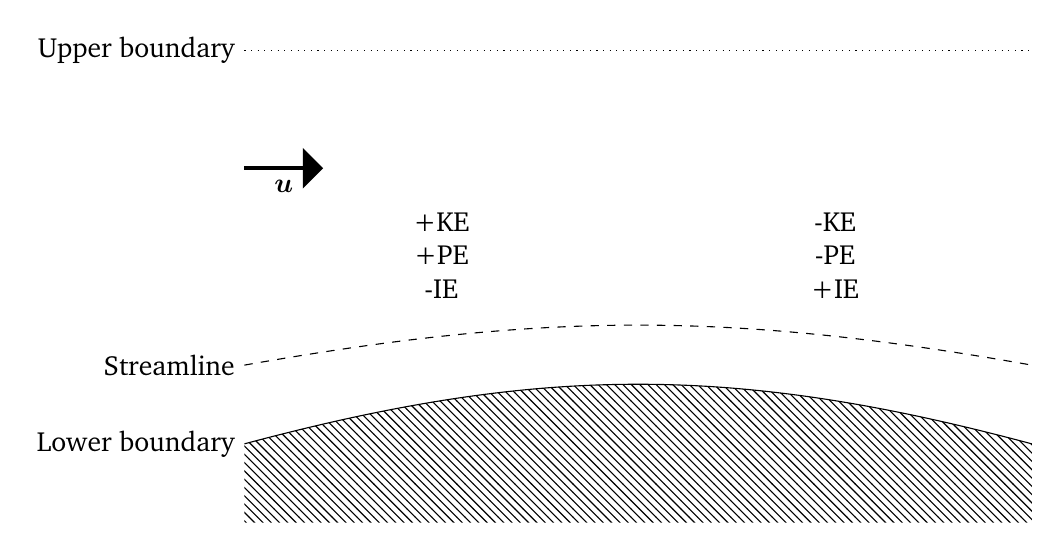
\begin{tikzpicture}
	\fill [pattern=north west lines] (0,0) to [bend left=15] (10,0) -- (10,-1) -- (0,-1);
	\draw (0,0) to [bend left=15] (10,0) node [at start, anchor=east] {Lower boundary};
	\draw [dotted] (0,5) -- (10,5) node [at start, anchor=east] {Upper boundary};
	\draw [dashed] (0,1) to [bend left=10] (10,1);
	\node [anchor=east] at (0,1) {Streamline};
	\node [anchor=south] at (2.5,1.6) {\makecell[c]{+KE\\+PE\\-IE}};
	\node [anchor=south] at (7.5,1.6) {\makecell[c]{-KE\\-PE\\+IE}};
	\draw [->, >=triangle 90, ultra thick] (0,3.5) -- (1,3.5) node [midway, below] {$\bm{u}$};
	\end{tikzpicture}
	\caption{Fluid flowing from left to right over a hill.  Following a streamline, kinetic energy (KE), potential energy (PE) increase and internal energy (IE) decreases as the pipe narrows on the windward side of the hill.  The reverse is true as the pipe widens on the lee side of the hill.}
	\label{fig:pipe}
\end{figure}

Given the incompressible, steady state flow, the flux across the inlet boundary, outlet boundary, or any vertical cross section through the interior, must be equal.  Hence, the fluid speed must be larger above the hill (or, conceptually, in the region of the constriction in the pipe).  The fluid must also gain gravitational potential energy as it ascends over the hill.  Bernoulli's principle then tells us that, in order to conserve energy, the pressure must decrease in the region above the hill.  Since pressure is proportional to temperature in an incompressible fluid, then temperature also decreases above the hill.

A few thoughts arise following on from this discussion:
\begin{itemize}
	\item Tracing streamlines that start at different heights we find that streamlines near the lower boundary will have greater changes in potential energy than streamlines near the upper boundary.  If this is true, then pressure and temperature will decrease the most following streamlines at the ground of the hill, and neither pressure nor temperature will vary along the upper boundary.
	\item We should look at our numerical model results and diagnose pressure and temperature fields from the prognostic variables.  Hydrostatic balance means pressure will vary with height as well as due to Bernoulli's principle, so we should subtract the hydrostatic pressure field in order to look only at the perturbation pressure field.
	\item How does potential temperature vary?  Recall that potential temperature, $\theta = T \left( p_0 / p \right)^{R/c_p}$.
	\item Can we explain the fluid behaviour using the Euler equations?
	\item How does the fluid behave if we consider that the upper boundary is a free surface?  Then Bernoulli's principle of energy conservation through a pipe no longer applies.
\end{itemize}
Some other ideas for further consideration:
\begin{itemize}
	\item How does a stratified fluid behave?  How can we explain the perturbations to potential temperature and vertical velocity that we've seen in two-dimensional numerical simulations?
	\item Think about flow regimes in relation to the Froude number.  How is this derived, what is the threshold value and why?
\end{itemize}


\bibliographystyle{ametsoc2014}
\bibliography{references}

\end{document}
